\section{Density of edge scoring for yeast data}


\begin{figure}[ht]
\centering
\begin{subfigure}[b]{\histwidth}\centering\caption{}
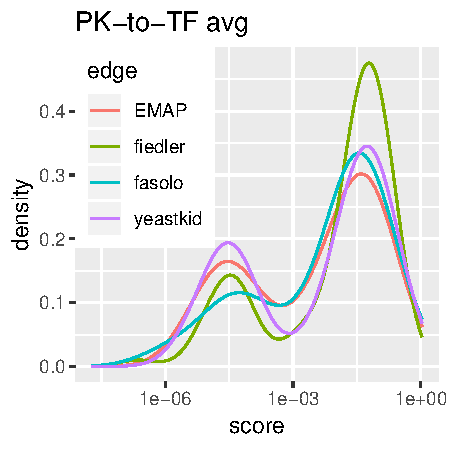
\includegraphics[width=\textwidth]{analysis/fig/hist_pk-tf_high_avg.pdf}
\end{subfigure}
\quad
\begin{subfigure}[b]{\histwidth}\centering\caption{}
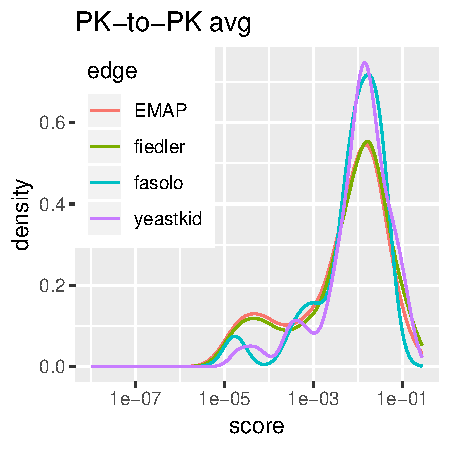
\includegraphics[width=\textwidth]{analysis/fig/hist_pk-pk_high_avg.pdf}
\end{subfigure}
\vskip\baselineskip
\begin{subfigure}[b]{\histwidth}\centering\caption{}
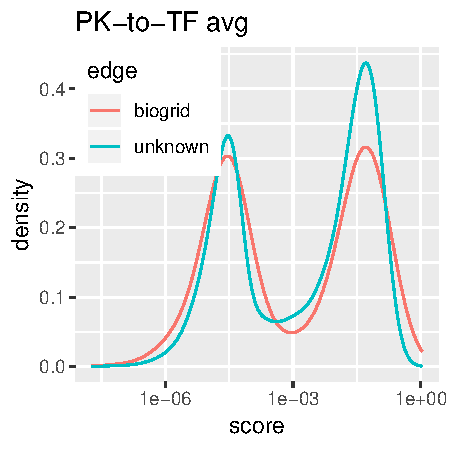
\includegraphics[width=\textwidth]{analysis/fig/hist_pk-tf_avg.pdf}
\end{subfigure}
\quad
\begin{subfigure}[b]{\histwidth}\centering\caption{}
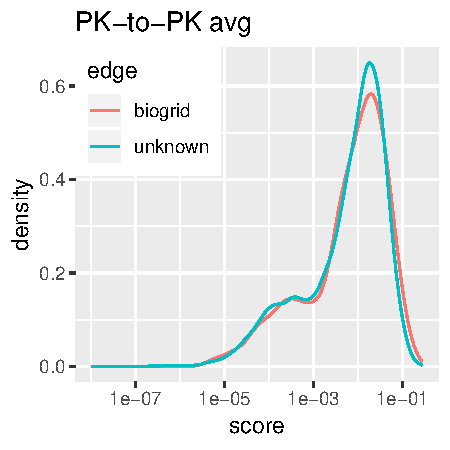
\includegraphics[width=\textwidth]{analysis/fig/hist_pk-pk_avg.pdf}
\end{subfigure}
\caption{\textbf{PK-to-PK and PK-to-TF for averaged edge inference attempts on yeast data.} Score as predicted weight value for edges from each dataset. Contrasted between high confidence edges~(a,b) and unknown and less likely edges~(c,d). "unknown" refers to possible edges not found in any of the datasets. x-axes are log10 scaled. }
\label{fig:yeast_hist_avg}
\end{figure}



\begin{figure}[ht]
\centering
\begin{subfigure}[b]{\histwidth}\centering\caption{}
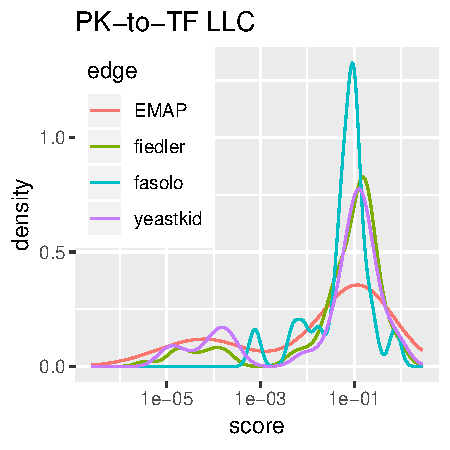
\includegraphics[width=\textwidth]{analysis/fig/hist_pk-tf_high_LLC.pdf}
\end{subfigure}
\quad
\begin{subfigure}[b]{\histwidth}\centering\caption{}
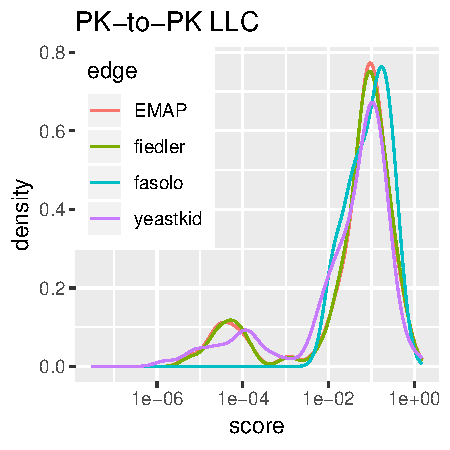
\includegraphics[width=\textwidth]{analysis/fig/hist_pk-pk_high_LLC.pdf}
\end{subfigure}
\vskip\baselineskip
\begin{subfigure}[b]{\histwidth}\centering\caption{}
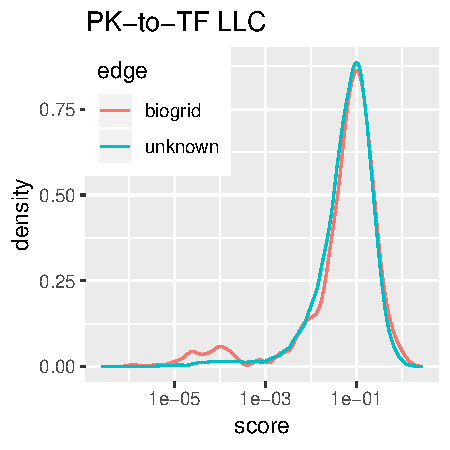
\includegraphics[width=\textwidth]{analysis/fig/hist_pk-tf_LLC.pdf}
\end{subfigure}
\quad
\begin{subfigure}[b]{\histwidth}\centering\caption{}
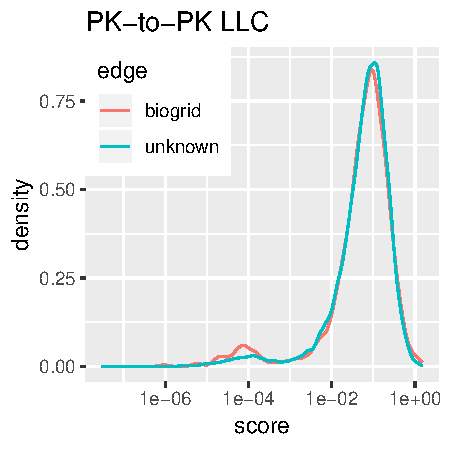
\includegraphics[width=\textwidth]{analysis/fig/hist_pk-pk_LLC.pdf}
\end{subfigure}
\caption{\textbf{PK-to-PK and PK-to-TF for LLC edge inference attempt on yeast data.} Score as predicted weight value for edges from each dataset. Contrasted between high confidence edges~(a,b) and unknown and less likely edges~(c,d). "unknown" refers to possible edges not found in any of the datasets. x-axes are log10 scaled. }
\label{fig:yeast_hist_llc}
\end{figure}

